\documentclass{article}

\usepackage[margin = 3cm, footskip = 30pt]{geometry}
\usepackage{amsmath}
\usepackage{tikz}
\usepackage{amssymb}
\usepackage{pgfplots}
 


\title{Linear Algebra (Part 002)\\Understanding Simultaneous System of Linear Equations}
\author{Dr. Kapil\\Department of Computer Applications\\ NIT Kurukshetra}
\date{\today}

\begin{document}
\maketitle
In the first part, we tried to understand vectors. And we said it many times that the property of remain in the same set after being operated is called \textit{closure} property. And we have seen that $\mathbb{R}^n$ is closed over vector addition and scalar multiplication.\\

Now, let us see these vector in some real problem.\\

\section{System of Linear Equations}\label{first_section}
    Example : \\

A company produces $N_1$, \ldots, $N_n$ for which resource $R_1$, \ldots, $R_m$ are required. To produce a unit of product $N_j$, $a_{ij}$ units of resource $R_i$ are required, where $1 \leq i \leq m$ and $1 \leq j \leq n$. It is known that we have exactly $b_i$ units of resources $R_i$. So what could be the plan i.e. quantity of products should be produced so that nothing is left behind.\\

Let $x_j$ be the number of units produced according to the plan for the product $N_j$. Thus, the total consumption of $R_i$ in producing $a_{ij}x_j$. And total consumption of the resource $R_i$ in producing $x_1,x_2,\ldots,x_n$ units of products $N_1$, \ldots, $N_n$ is $a_{i1}x_1 + a_{i2}x_2 + \ldots + a_{in}x_n$. To ensure no wastage, we have to equate it with total available quantity of resource $R_i$ (i.e. $b_i$). Hence,
\begin{align}
   a_{i1}x_1 + a_{i2}x_2 +\ldots+ a_{in}x_n & = b_i\nonumber
\end{align}

Thus, all the units $b_i$ of resources $R_i$ are utilized in the production of $x_j$ units of $N_j$ product for all $j\in{1,2,\ldots,n}$. That is-\\
\begin{align}
    a_{11}x_1 + a_{12}x_2 + \ldots + a_{1n}x_n &= b_1\nonumber\\
    a_{21}x_1 + a_{22}x_2 + \ldots + a_{2n}x_n &= b_2\nonumber\\
    &\vdots\nonumber\\
    a_{m1}x_1 + a_{m2}x_2 + \ldots + a_{mn}x_n &= b_n\nonumber
\end{align}

When a particular value of \((x_1, x_2, \ldots, x_n)\) solves all the equations that solution of system. This is also known as simultaneous set of linear equations. That is all the equality's should hold for the same value of \((x_1, x_2, \ldots, x_n) \in \mathbb{R}^n\).\\

Now, instead of trying to understand such a big system. Let us talk about smaller and concrete system.\\
Case 1:\\
\begin{align}
    x_1 + x_2 &= 2 &&  \text{(L1)}\label{L1}\\
    x_1 - x_2 &= 0 &&  \text{(L2)}\label{L2}
\end{align}

Clearly, both the equality's are satisfied when $x_1 = 1$ and $x_2 = 1$. If you see them graphically any point on \(L_1\) satisfies equation(\ref{L1}) and any point on \(L_2\) satisfies equation(\ref{L2}). And the intersection point is the one which satisfies both equation(\ref{L1}) and equation(\ref{L2}).\\

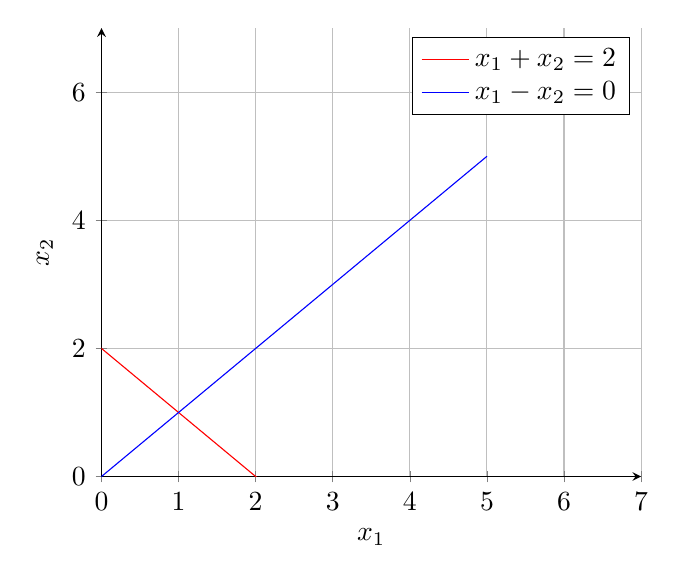
\begin{tikzpicture}
    \begin{axis}[
        grid=both,
        axis lines = left,
        xlabel = $x_1$,
        ylabel = $x_2$,
        xmin=0, xmax=7,
        ymin=0, ymax=7,
    ]
        \addplot [color=red]{2-x};
        \addlegendentry{$x_1 + x_2 = 2$}
        \addplot [color=blue]{x};
        \addlegendentry{$x_1 - x_2 = 0$}
    
    \end{axis}
\end{tikzpicture}

Case 2:\\

\begin{align}
    x_1 + x_2 &= 2 &&  \text{(L3)}\label{L3}\\
    2x_1 + 2x_2&= 4 &&  \text{(L4)}\label{L4}
\end{align}

Keeping $x_1, x_2$ on the same side of equality and dividing the equation(\ref{L4}) by 2 throughout, we get to know that both the equations \ref{L3} and \ref{L4} represents same thing. Therefore, any point $(a, 2-a) \forall a \in \mathbb{R}^n$ will satisfy both the equations. And this `$a$` can take infinitely many values. So, we have infinitely many solutions. And graphically, they mean both the line overlap and hence provide infinite number of solution that can satisfy both the equations simultaneously.\\

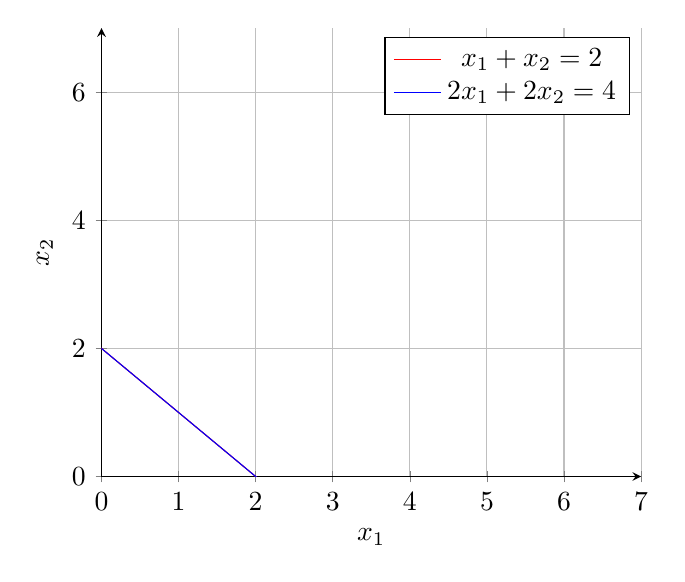
\begin{tikzpicture}
    \begin{axis}[
        grid=both,
        axis lines = left,
        xlabel = $x_1$,
        ylabel = $x_2$,
        xmin=0, xmax=7,
        ymin=0, ymax=7,
    ]
        \addplot [color=red]{2-x};
        \addlegendentry{$x_1+x_2 = 2$}
        \addplot [color=blue]{2-x};
        \addlegendentry{$2x_1+2x_2 = 4$}
    \end{axis}
\end{tikzpicture}

Case 3:\\

\begin{align}
    x_1 + x_2 &= 2 &&  \text{(L5)}\label{L5}\\
    2x_1 + 2x_2 &= 5  &&  \text{(L6)}\label{L6}
\end{align}

Obviously, when you multiply first by $2$, then for any value of \((x_1, x_2)\), that satisfies equation(\ref{L5}) cannot satisfy equation(\ref{L6}). Thus, we cannot have a common solution among them. Graphically, it means they can not meet.\\

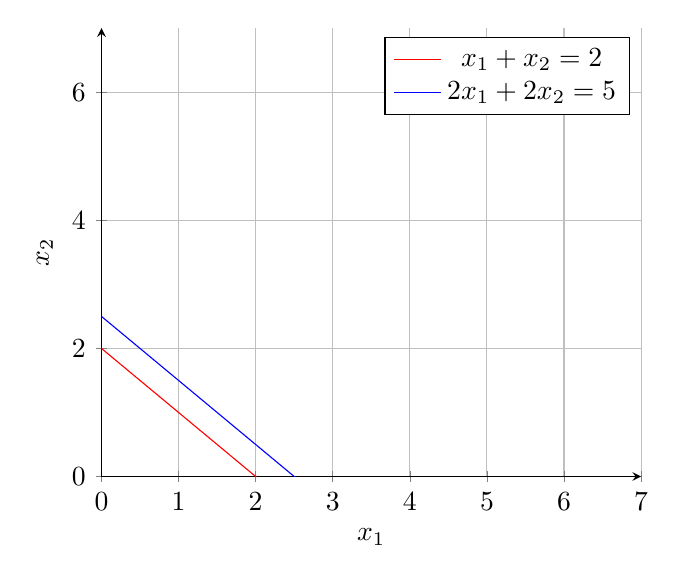
\begin{tikzpicture}
    \begin{axis}[
        grid=both,
        axis lines = left,
        xlabel = $x_1$,
        ylabel = {$x_2$},
        xmin=0, xmax=7,
        ymin=0, ymax=7,
    ]
        \addplot [color=red]{2-x};
        \addlegendentry{$x_1 + x_2 = 2$}
        \addplot [color=blue]{(5 - 2*x) / 2};
        \addlegendentry{$2x_1 + 2x_2 = 5$}
    \end{axis}
\end{tikzpicture}

You can try to generate the similar case for 3 variable equations. [refer to mml-book page 20.]\\

Conclusion:\par
Any real valued system of linear equations has either no, exactly one, or infinitely many solutions. Now, let us look Case 1 \textbf{Unique Solution} in different way.\\
\begin{align}
    x_1 + x_2 &= 2 \nonumber\\
    x_1 - x_2 &= 0 \nonumber
\end{align}

\[
\implies x_1 \begin{pmatrix}
                1\\
                1\\
             \end{pmatrix} + x_2 \begin{pmatrix}
                1\\
                -1\\
            \end{pmatrix} = \begin{pmatrix}
                2\\
                0\\
            \end{pmatrix}
\]

We have only one equation but involving 2D vector \(\vec{v_1}\) and \(\vec{v_2}\). Now, what does this mean?\\
Let's go back to our vector operation\\
\begin{enumerate}
    \item Scalar multiplication - It scales the vector by some scalar quantity\\
\[  ex.~ \vec{u_1} = \begin{pmatrix}
                                1\\
                                2\\
                            \end{pmatrix}, ~ 2\times \vec{u}= 2\begin{pmatrix}
                                1\\
                                2\\
                             \end{pmatrix} = \begin{pmatrix}
                                2\\
                                4\\
                            \end{pmatrix}
\]

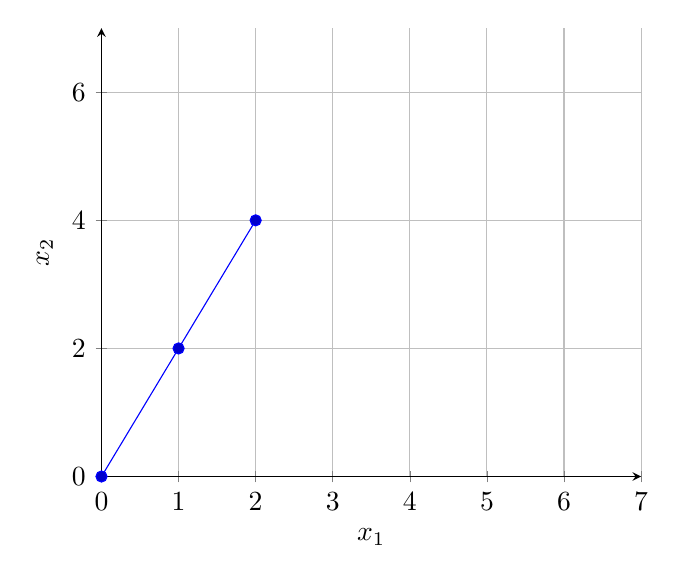
\begin{tikzpicture}
    \begin{axis}[
        grid=both,
        axis lines = left,
        xlabel = $x_1$,
        ylabel = {$x_2$},
        xmin=0, xmax=7,
        ymin=0, ymax=7,
    ]
        \addplot coordinates {(0,0) (1, 2) (2, 4)};
    \end{axis}
\end{tikzpicture}


Graphically, it is just changing the magnitude of the vector.
    
    \item Addition of two vector 
    
\[
    \vec{u} = \begin{pmatrix}
                    1\\
                    1\\
               \end{pmatrix}, \vec{v} = 
               \begin{pmatrix}
                    1\\
                    -1\\
               \end{pmatrix}
\]    




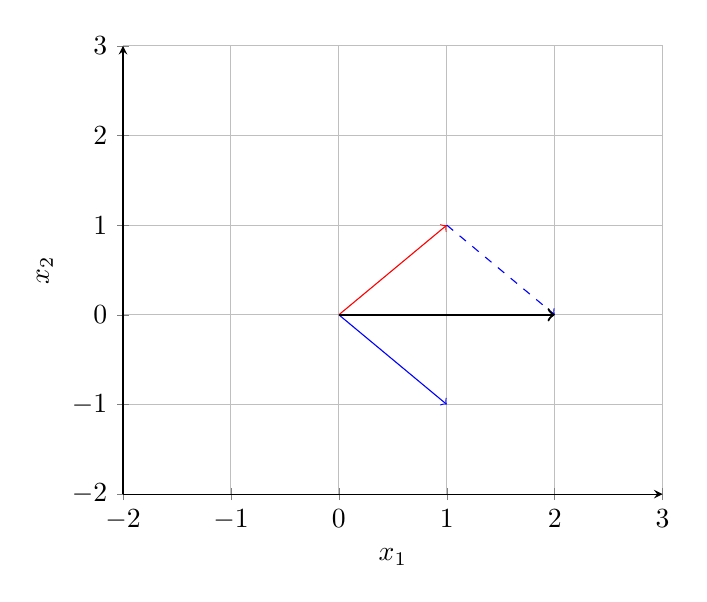
\begin{tikzpicture}
    \begin{axis}[
        grid=both,
        axis lines = left,
        xlabel = $x_1$,
        ylabel = $x_2$,
        xmin=-2, xmax=3,
        ymin=-2, ymax=3,
        after end axis/.code={
               \draw[red,->] (axis cs:0,0) -- (axis cs:1,1);
               \draw[blue,->] (axis cs:0,0) -- (axis cs:1,-1);
               \draw[dashed,blue,->] (axis cs:1,1) -- (axis cs:2,0);
               \draw[thick, black,->] (axis cs:0,0) -- (axis cs:2,0);
               }
    ]
    \end{axis}
\end{tikzpicture}
\end{enumerate}

Put the tail of one vector on to the head of the another and now whatever location you are pointing to, is the resultant vector.\\

Now going back to case 1\\

\[
    x_1 \begin{pmatrix}
            1\\
            1\\
        \end{pmatrix} + x_2 \begin{pmatrix}
                                1\\
                                -1
                            \end{pmatrix} = \begin{pmatrix}
                                                2\\
                                                0
                 \end{pmatrix}
\]

So, this equation asks for what scaling factor of the vectors followed by their addition can generate the vector \( \begin{pmatrix}
                2\\
                0
              \end{pmatrix} \)?\\

The sequence of scalar multiplication and addition of vectors is called Linear Combination. So, the question what is the right Linear Combination of \(\begin{pmatrix}1\\ 1\\\end{pmatrix}\text{ and }\begin{pmatrix}
                                      1\\
                                      -1
             \end{pmatrix}\) that can make \(\begin{pmatrix}
                            2\\
                            0
            \end{pmatrix}\).
                                                     
Further you can see in following way \(\begin{pmatrix}
                            1 & 1\\ 
                            1 & -1 
                     \end{pmatrix} \begin{pmatrix}
                            x_1\\
                            x_2
                    \end{pmatrix} = \begin{pmatrix}
                                2\\
                                0
                    \end{pmatrix}\). This can be rewritten as \(A\vec{x} = \vec{b},\text{ where, }A = \begin{pmatrix}
                            1 && 1\\
                            1 && -1\\
                        \end{pmatrix}\), a matrix of order $2\times 2$; $\vec{x}$ is a unknown vector and $2\times1~\vec{b}$ is a known vector.




\section{Exercise (Homework)}

Extend Linear Combination view (or Understanding) for the other two cases. That means we need to understand how vector form of equations will see the no solution, and infinitely many solution cases.\\ \\
Case \textbf{Infinitely Many Solutions}:
\begin{align}
    x_1 + 2x_2 = 2 \nonumber\\
    2x_1 + 4x_2 = 4  \nonumber
\end{align}
Its vector view is like this
\begin{align}
    \begin{bmatrix}
    1\\2
    \end{bmatrix} \times x_1 +
    \begin{bmatrix}
    2\\4
    \end{bmatrix} \times x_2 = 
    \begin{bmatrix}
    2\\4
    \end{bmatrix} \nonumber
\end{align}
which means that sum of vectors with same direction are making another vector in that direction and you can do it in many ways. Fix $x_2$ and value of $x_1$ can be found to satisfy the equation.
can be rewritten as -
\begin{align}
    \begin{bmatrix}
    1\\2
    \end{bmatrix} \times (x_1 +2x_2)=\begin{bmatrix}
    2\\4
    \end{bmatrix} \nonumber
\end{align}

Case \textbf{No Solution}:
\begin{align}
    x_1 + x_2 = 2 \nonumber\\
    2x_1 + 2x_2 = 5  \nonumber
\end{align}
Its vector view is like this
\begin{align}
    \begin{bmatrix}
    1\\2
    \end{bmatrix} \times x_1 +
    \begin{bmatrix}
    1\\2
    \end{bmatrix} \times x_2 = 
    \begin{bmatrix}
    2\\5
    \end{bmatrix} \nonumber
\end{align}
which is equivalent to ask for sum of the two vectors with same direction to make a vector in different direction. Its impossible as you can only remain in that direction as you are just scaling a vector. The system can be rewritten as -
\begin{align}
    \begin{bmatrix}
    1\\2
    \end{bmatrix} \times (x_1 +x_2)=\begin{bmatrix}
    2\\5
    \end{bmatrix} \nonumber
\end{align}
So you cannot generate vector that is in another direction if the given vector are in same direction.
\end{document}